\chapter{ObjectProxyFactory}
The \textit{ObjectProxyFactory} creates \textit{ObjectProxy} instances with \textit{TDataMember} type, \textit{TClassRef} scope and \textit{ObjectProxy} holder. It encapsulates ROOT objects recursively for use in JavaScript.\\

To handle cyclical references a cache of already generated \textit{ProxyObject}s will be maintained, which will only be valid during object conversion. When an object is cached it will be used instead of creating a new one.
\begin{figure}[H]
	\centering
	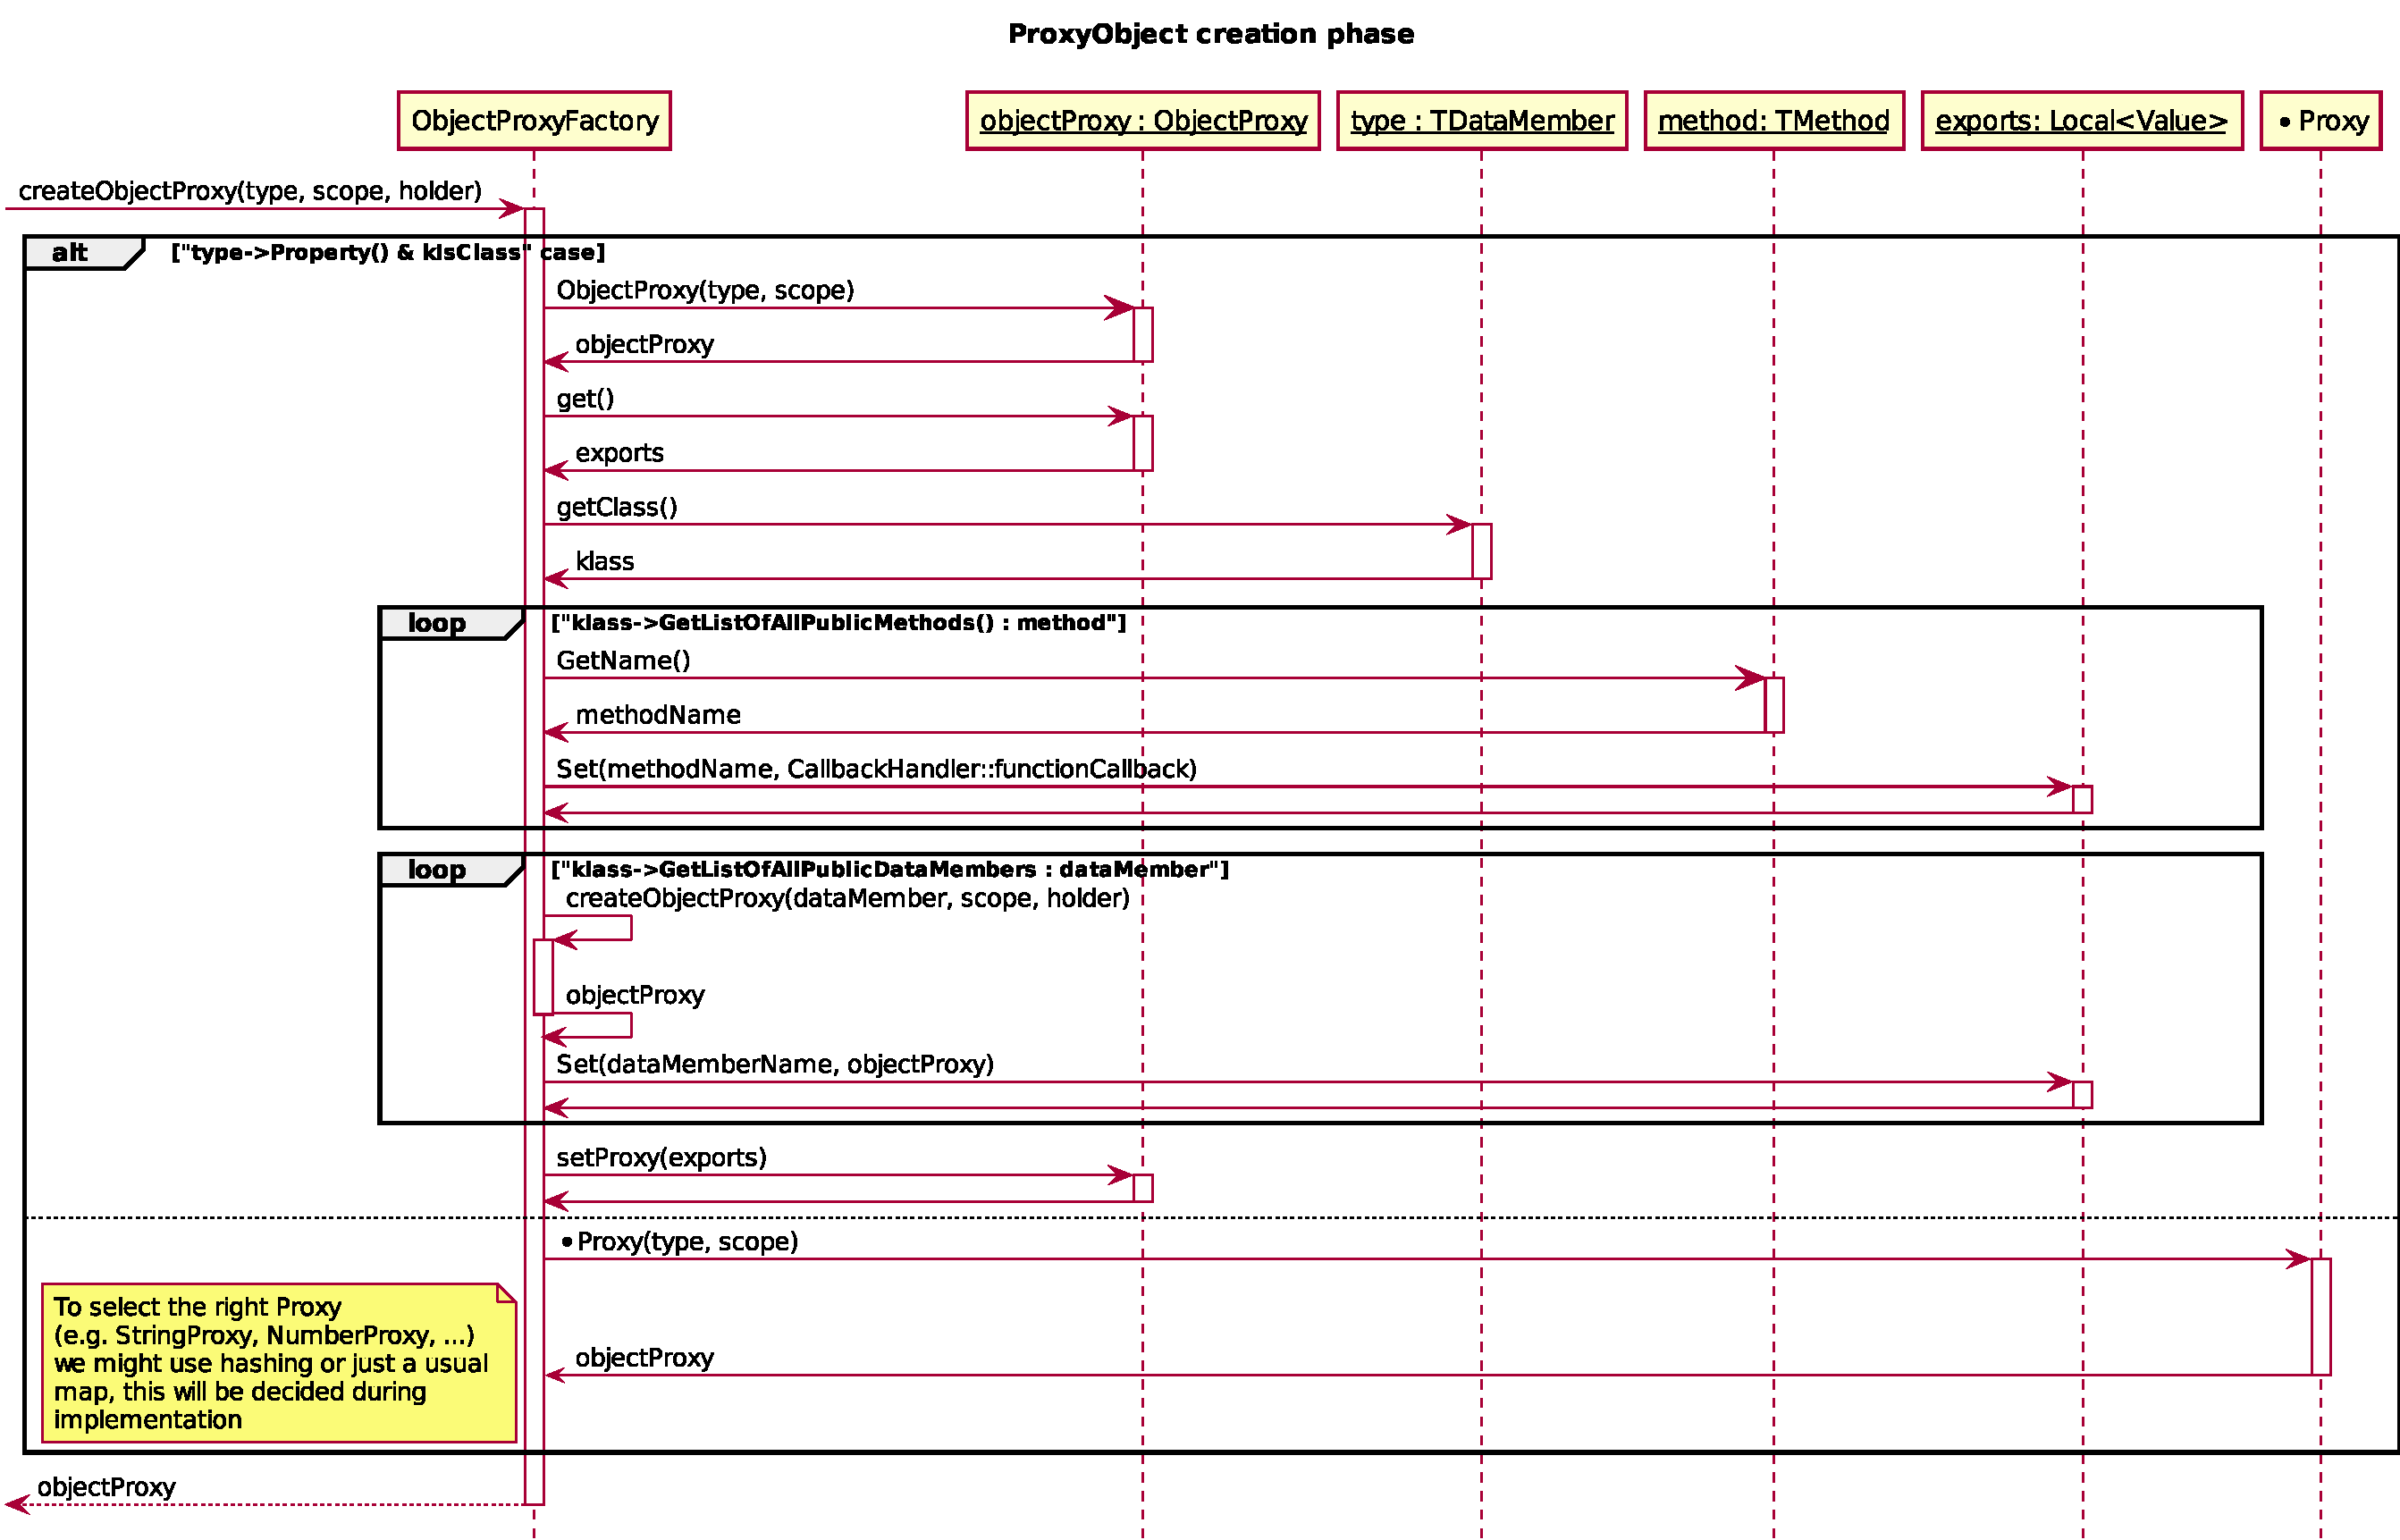
\includegraphics[width=18cm]{./latex/resources/createProxyObject.pdf}
	\caption{object proxy creation sequence}
\end{figure} \pagebreak
\section{createObjectProxy}
\begin{longtable}{p{3cm} @{\hskip 1cm} p{12cm}}
 \hline
\textit{Name} & \texttt{ObjectProxyFactory::createObjectProxy(type: TDataMember, scope: TClassRef, holder: ObjectProxy)}\\
\hline
 \textit{Visibility} & public\\
\hline
\textit{Parameters} & \textit{type: TDataMember} The type identification which the ObjectProxy will have \\
& \textit{scope: TClassRef} The class the ObjectProxy belongs to \\
& \textit{holder: ObjectProxy}  The holder is the ObjectProxy which will encapsulate and hold the newly created ObjectProxy \\
\hline
\textit{Return value} & \textbf{ObjectProxy} Returns the ObjectProxy which is created with the given parameters.\\
  \hline
 \textit{Behavior} & A new ObjectProxy is created each time the createObjectProxy method is called up. \\
\hline
\end{longtable} \pagebreak
